\documentclass[chaptersright]{informeutn}
\usepackage{circuitikz}

% Datos del informe
\materia{Electrónica Aplicada I}
\titulo{Trabajo Práctico 3}
\comision{3R2}
\autores{
          Gaston Grasso - 401892\\
          Franco Palombo - 401910\\
          Angelo Prieto - 401012}
\fecha{20/08/2025}

\begin{document}
  \maketitle

  \tableofcontents
  \setcounter{page}{1}
  \thispagestyle{plain}

\chapter{Diseño para Máxima Excursión Simétrica}
  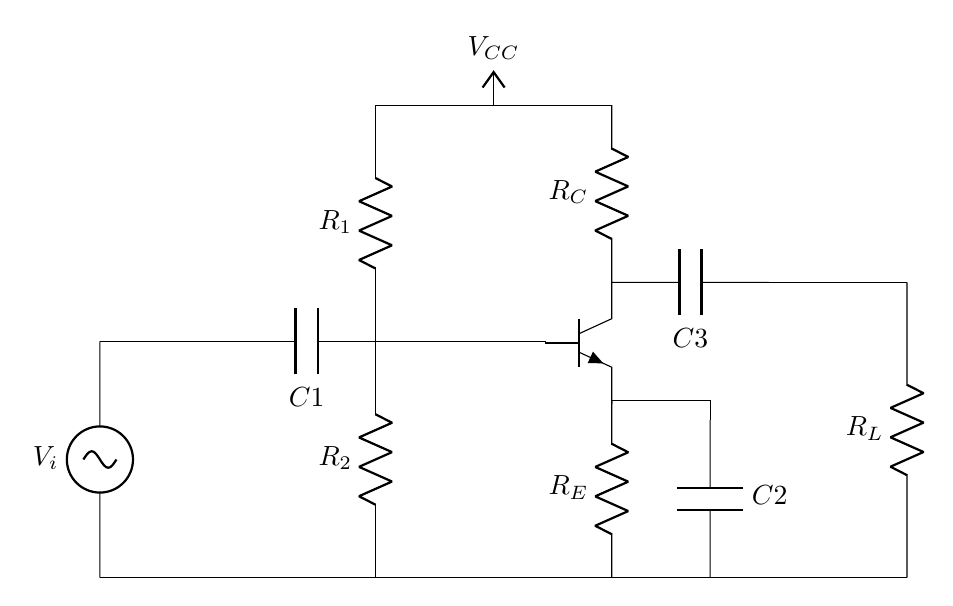
\begin{tikzpicture}
	% Paths, nodes and wires:
	\node[npn] at (7, 5.98){};
	\draw (6.16, 5.98) |- (4, 6);
	\draw (4, 6) to[american resistor, l={$R_1$}, label distance=0.02cm] (4, 9);
	\draw (4, 3) to[american resistor, l={$R_2$}, label distance=0.02cm] (4, 6);
	\draw (7, 6.75) to[american resistor, l={$R_{C}$}, label distance=0.02cm] (7, 9);
	\draw (7, 3) to[american resistor, l={$R_{E}$}, label distance=0.02cm] (7, 5.25);
	\draw (0.5, 3) to[sinusoidal voltage source, l={$V_i$}, label distance=0.02cm] (0.5, 6);
	\draw (4, 6) to[capacitor, l={$C1$}, label distance=0.02cm] (2.25, 6);
	\draw (2.25, 6) |- (0.5, 6);
	\draw (0.5, 3) -- (4, 3);
	\draw (8.25, 5) to[capacitor, l={$C2$}, label distance=0.02cm] (8.25, 3);
	\draw (8.25, 5) |- (7, 5.25);
	\draw (8.25, 3) |- (7, 3);
	\draw (4, 3) -- (7, 3);
	\draw (4, 9) -- (7, 9);
	\draw (5.5, 9) -- (5.5, 9);
	\draw (9, 6.75) to[capacitor, l={$C3$}, label distance=0.02cm] (7, 6.75);
	\node[vcc](N1) at (5.5, 9){} node[anchor=south] at ([yshift=0.03cm]N1.north){$V_{CC}$};
	\draw (10.75, 3) to[american resistor, l={$R_{L}$}, label distance=0.02cm] (10.75, 6.75);
	\draw (10.75, 6.75) -- (9, 6.75);
	\draw (8.25, 3) -- (10.75, 3);
\end{tikzpicture}
  \section{Enunciado y datos iniciales}
    % Copiar aquí el planteo y los datos (RE, RC, RL, elección de transistor y VCC)
  \section{Cálculo de R1 y R2}
    \subsection{Teorema de Thévenin en red de entrada}
    \subsection{Análisis de malla de entrada}
    \subsection{Criterios de diseño y fórmulas generales}
    \subsection{Cálculo final de R1 y R2}
  \section{Simulación}
    \subsection{Simulación con valores de diseño}
    \subsection{Simulación con valores normalizados}
    \subsection{Comparación con cálculos analíticos}
  \section{Implementación y mediciones}
    \subsection{Mediciones en circuito implementado}
    \subsection{Consideraciones de medición}
    \subsection{Cálculo de parámetros a partir de mediciones}

\chapter{Análisis y trazado de rectas de carga}
  \section{Recta de carga en corriente continua (CC)}
    \subsection{Ecuación y puntos de corte}
  \section{Recta de carga en corriente alterna (CA)}
    \subsection{Ecuación y puntos de corte}
  \section{Obtención experimental de parámetros}
    \subsection{Corrientes en el divisor resistivo}
    \subsection{Verificación de resultados}

\chapter{Mediciones de pequeña señal}
  \section{Análisis teórico (método analítico)}
    \subsection{Circuito híbrido equivalente}
    \subsection{Cálculo de $Z_i$, $Z_o$, $A_i$ y $A_v$}
  \section{Análisis experimental}
    \subsection{Impedancia de entrada}
    \subsection{Ganancia de tensión}
    \subsection{Ganancia de corriente}
    \subsection{Impedancia de salida}


\end{document}
